\section{Problem}

In \pcc{}, we have a set of $n$ objects and a binary relationship denoting
similarity $(+)$  or dissimilarity $(-)$ between these objects. Such data are
naturally associated with a signed graph $G=(V,E)$. The objective is to
cluster them according to this similarity information.

In this clustering problem, the number of clusters is part of the solution as
opposed of being an input constraint, which is sometime desirable in
unsupervised setting. Furthermore, it does not require a distance between
points (although such extra information can be taken into account through
edges weight).

Given any node partition, a \emph{disagreements edge} is a positive edge within a
cluster or a negative edge between different clusters. A natural complexity
measure for the edge labeling (the signs associated with edges) is the minimum
number of disagreement edges over \textbf{all} possible node partitions of the node
set. The number of disagreements created by a given clustering is called its
cost.

\medskip

The problem of finding a partition minimizing the number of disagreements
edges was showed to be NP-hard, even on complete graph \autocite{Bansal2002}.
Yetthere exists an elegant algorithm by \textcite{Ailon2008} (referred
later as \ccp{}) that runs in $O(n\left|\mathcal{P}_{\text{\ccp{}}}\right|)$,
where $\left|\mathcal{P}_{\text{\ccp{}}}\right| \le |V|$ is the number of
clusters found with this strategy. It is a randomized algorithm with an
expected approximation ratio of $3$.

When the input is a general graph, the problem becomes APX-hard
\autocites{Charikar2003}{Demaine2006}, and these two papers provide polynomial
algorithms achieving $O(\log n)$ approximation. Yet they resort to expensive
semi definite programs so we are seeking a combinatorial approach that would
transform a graph into a clique, in order to apply the \ccp{} algorithm.

\section{Method}

A \emph{triangle} is any set of three distinct nodes, regardless of their
order. One triangle is \emph{closeable} if it satisfies the following
conditions:
\begin{enumerate}
	\item it has exactly two edges
	\item at least one edge is positive
\end{enumerate}
Such triangles have a special node called \emph{center} which is the endpoint
of the two edges (see \autoref{fig:triangle}).
\begin{figure}[htpb]
	\centering
	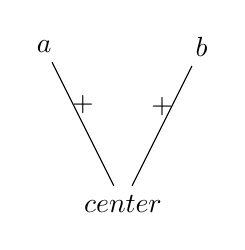
\begin{tikzpicture}[scale=.2]
		% inner sep=3pt,draw=Black,shape=circle
		\node[] (a) at (0,0) {$a$};
		\node[] (b) at (10,0) {$b$};
		\node[] (p) at (5,-10) {$center$};
		\draw[] (a) -- (p) node[midway,above] {$+$};
		\draw[] (b) -- (p) node[midway,above] {$+$};
	\end{tikzpicture}
	\caption{A closeable triangle \label{fig:triangle}}
\end{figure}

We obtain a clique by iteratively closing these triangles; by adding to them a
third edge whose sign is the product of the signs of the two existing edges.

The crucial decision is how to choose the triangles to close during the
current iteration. For that, we define a strategy as a pair of boolean
(\pvt{}, \oaat{}). If \pvt{} is true, we first select a vertex $p$ uniformly
at random from $V$ and we restrict candidate triangles to have $p$ as center.
Otherwise, we consider all possible closeable triangles as candidates.  Then,
if \oaat{} is true, we select one triangle uniformly at random from the
candidates, otherwise we select all of them. These four strategies are named
in \autoref{tab:strategy} and the procedure just discussed is formally
described below as \textsc{PickTriangles}, where $C$ is the set of all
currently closeable triangles in $G$.

\begin{center}
	\rule{\textwidth}{.3pt}
	% \caption{Selecting some triangles to be closed \label{alg:pick}}
	\begin{algorithmic}[0]
		\Function{\textsc{PickTriangles}}{$G=(V,E),\,strategy,\, C$}
			\If{$strategy.$\pvt{}}
				\Let{$pivot$}{one element from $V$ selected uniformly at
					random}
				\Let{$candidates$}{$\{t \in C : center(t) = pivot\}$}
			\Else
				\Let{$candidates$}{$C$}
			\EndIf
			\If{$strategy.$\oaat{}}
				\State \textbf{return} a element of $candidates$ uniformly at
				random 
			\Else
				\State \textbf{return} $candidates$
			\EndIf
		\EndFunction
	\end{algorithmic}
	\rule{\textwidth}{.3pt}
\end{center}

\begin{table}[hptb]
	\centering
	\caption{Short names of the different randomization strategy
		\label{tab:strategy}}
	\begin{tabular}{lccc}
		\toprule
		& & \multicolumn{2}{c}{\pvt{}} \\
		    &          & True & False \\
		\midrule
		\multirow{2}{*}{\oaat{}} & True   & $P_1$ & $N_1$ \\
		& False & $P_*$ & $N_*$ \\
		\bottomrule
	\end{tabular}
\end{table}

The full algorithm is presented in \autoref{alg:complete}. Its input is a
graph $G$ with node set $V=\{0, 1,\ldots, n-1\}$ and edge set $E$.

\begin{algorithm}
	\caption{\textsc{Complete}($G=(V,E),\,strategy$) \label{alg:complete}}
	\begin{algorithmic}[0]
		\State \emph{Note:} in the following, $triangle = (a, center, b)$, as
			shown in \autoref{fig:triangle}
		\Let{$C$}{$\emptyset$}
		\ForAll{$triplets$ of distinct nodes $(a,v,b)$ in $V^3$}
		\If{$(a,v,b)$ is a closeable triangle}
			\Let{$C$}{$C \cup \{(a,v,b)\}$}
		\EndIf
		\EndFor
		\While{$C \neq{} \emptyset$}
		\Let{$just\_closed$}{$\emptyset$}
			\ForAll{$triangle$ in \textsc{PickTriangles}$(C)$}
				\State \textsc{Close}$(triangle)$
				\Let{$just\_closed$}{$just\_closed \cup \{triangle\}$}
			\EndFor
			\ForAll{$triangle$ in $just\_closed$}
			\State \textsc{Update}$(C,\, triangle)$
			\EndFor
		\EndWhile
		\State set remaining edges to negative
		% \EndFunction
		\vspace*{0.5\baselineskip}
		\begin{center}
			\rule{0.5\textwidth}{.2pt}
		\end{center}
		\vspace*{0.5\baselineskip}

		\Function{\textsc{Close}}{$triangle$} 
		\State add edge $(a, b)$
		\Let{$sign(a, b)$}{$sign(a, center) \times sign(center, b)$}
		\EndFunction
		\vspace*{\baselineskip}
		\Function{\textsc{Update}}{$C,\, triangle=(a, center, b)$}
			\Let{$N_a$}{neighbors of $a$}
			\Let{$N_b$}{neighbors of $b$}
			\ForAll{$v \in \left(N_a \cap N_b\right)\setminus \{a,b\}$}
				\Let{$C$}{$C \setminus \{(a, v, b)\}$}
			\EndFor
			\ForAll{$v \in N_a$}
				\If{$(v, a, b)$ is closeable}
					\Let{$C$}{$C \cup \{(v, a, b)\}$}
				\EndIf
			\EndFor
			\ForAll{$v \in N_b$}
				\If{$(v, b, a)$ is closeable}
					\Let{$C$}{$C \cup \{(v, b, a)\}$}
				\EndIf
			\EndFor
		\EndFunction
	\end{algorithmic}
\end{algorithm}

\section{Experiment}

We try our implementation on different controlled geometries to see how it
behaves. Most of them involve \emph{bad cycle}, that is cycle with exactly one
negative edge that will necessarily incurs at least one disagreement.  Because
our algorithm is randomized, we complete each graph 50 times.  On each
completed graph, we run the \ccp{} algorithm 100 times, to obtain an
estimation of the expected cost of the complete graph. In all the following
tables, we report the number of disagreement edges among edges of the original
graph.

\subsection{One bad cycle of length $n$}
\label{sub:cycle}

The optimal solution is either one or two connected clusters, yielding one
disagreement. Strategy \pat{} achieves this optimum while \pot{} number of
errors grows linearly with the length $n$ of the cycle. The same is true when
we do not select pivot. (the missing number are due to lack of time).

\begin{center}
\begin{tabular}{lrrrrrrrrr}
\toprule
$n$      & 8   & 16  & 32  & 64   & 128  & 256  & 384   & 512   & 1024 \\
\midrule
\pot{}   & 1.4 & 3.1 & 7.3 & 17.2 & 40.0 & 86.2 & 132.7 & 179.6 & 371.0 \\
\pat{}   & 1.0 & 1.0 & 1.0 & 1.0  & 1.0  & 1.0  & --    & --    & -- \\
\nnot{}  & 1.4 & 2.6 & 5.1 & 7.3  & 11.2 & 17.9 & --    & --    & --\\
\nat{}   & 1.0 & 1.0 & 1.0 & 1.0  & 1.0  & 1.0  & --    & --    & --\\
\bottomrule
\end{tabular}
\end{center}



\subsection{Cycle of length 100 having only two negative edges separated by
	$k$ vertices}
Because there is more than one negative edge, the optimal solution cost is 0.
It is found consistently by both strategies.

\begin{center}
\begin{tabular}{lrrrrr}
\toprule
$k$ &   0  &   1  &   25 &   50  \\
\midrule
\pot{} & 0.0 & 0.0 & 0.0 & 0.0  \\
\pat{} &  0.0 &  0.0 & 0.0 & 0.0  \\
\bottomrule
\end{tabular}
\end{center}

\subsection{Bad squares sharing only one (positive) edge}
\label{sub:squares}
Here, the optimal solution is to create two clusters in the following ways.
Say the shared edge is between vertices $0$ and $1$. Each of these two
vertices is put in one cluster. Starting from $0$, we can follow a path on
every cycle and put vertices we cross in $0$'s cluster, until we encounter the
negative edge of the cycle. We do the same with $1$. The only disagreement is
the positive edge between $0$ and $1$, therefore the optimal cost is 1.

\begin{center}
\begin{tabular}{lrrrr}
\toprule
number of squares & 40   & 65   & 80    & 130 \\
\midrule
\pot{}            & 2.9  & 2.6  & 2.9   & 2.9 \\
\pat{}            & 24.1 & 42.8 & 53.4  & 76.2 \\
\nnot{}           & 49.9 & 84.8 & 108.6 & 184.2 \\
\nat{}            & 40.0 & 65.0 & 80.0  & 130.0\\
\bottomrule
\end{tabular}
\end{center}

Unfortunately, all but the \pot{} strategy fail to achieve this solution,
instead committing a number of errors linear with the number of bad cycles.


\subsection{Bad squares sharing only the (negative) edge}

If we move the position of the negative edge to the shared edge, the results
do not change.

\begin{center}
\begin{tabular}{lrrrrr}
\toprule
number of squares &  40  &  65  &  80  &  130 &  170 \\
\midrule
\pot{} &  2.0 &  1.9 &  2.1 &  4.6 &  2.0 \\
\pat{} & 21.8 & 31.7 & 42.6 & 62.6 & 88.2 \\
\bottomrule
\end{tabular}
\end{center}

\subsection{$\floor*{\sqrt{n}}$ bad cycles of length $\floor*{\sqrt{n}}$
	sharing one positive edge}
\label{sub:mixed}

Since the length of the cycle does not affect the optimal solution, its cost
is still $1$. But this case is challenging for all strategies.

\begin{center}
\begin{tabular}{lrrrrr}
\toprule
cycle length & 7    & 9    & 12   & 15   & 20 \\
\midrule
\pot{}       & 10.6 & 14.7 & 16.3 & 32.5 & 55.1 \\
\pat{}       & 6.8  & 8.8  & 12.0 & 15.1 & 20.1 \\
\nnot{}      & 17.2 & 23.9 & 32.2 & 41.6 & 58.7 \\
\nat{}       & 9.1  & 12.1 & 19.8 & 19.3 & 35.3 \\
\bottomrule
\end{tabular}
\end{center}


\subsection{Planted clustering}

We create $k$ clusters $\{C_1, \ldots, C_k\}$ of roughly the same size $n_i$
with around $2n$ positive edges inside them and $n_i\cdot n_j$ negative edges
across each others. Then we flip a fraction $p=0.07$ of edges at random.
Since $p$ is \enquote{small}, this give us an estimation of the optimal number
of disagreements, provided that the clustering stays the same. A similar model
is considered by \textcite{Makarychev2014}.

In the table below, we report the number of disagreements divided by the
number of flipped edges (because being random, all the graphs do not have the
same number of edges, making comparison unfair). If the original clustering
was not too much perturbed, this is an estimation of the approximation ratio
of our method.

\begin{center}
\begin{tabular}{lrrrrrrrrr}
\toprule
$k$      & 5   & 10  & 30  & 20  & 15  & 2   & 2   & 2   & 2  \\
$n$      & 15  & 25  & 6   & 12  & 35  & 20  & 40  & 65  & 100 \\
nodes    & 75  & 250 & 180 & 240 & 525 & 40  & 80  & 130 & 200 \\
\midrule
\pat{}   & 2.2 & 2.1 & 1.6 & 1.7 & 1.9 & 2.0 & 2.5 & 2.6 & 3.0 \\
\pot{}   & 3.2 & 2.8 & 1.7 & 2.0 & 2.4 & 4.5 & 5.9 & 6.5 & 7.0 \\
\bottomrule
\end{tabular}
\end{center}

\section{Discussion}

None of the strategy work well in all case. \pot{} is good for many squares
whereas \pat{} is optimal for one long bad cycle, and both fail in the middle
case of \autoref{sub:mixed}.

Yet by providing a little help to the algorithm, we can greatly reduce the
number of mistakes. Namely, if we avoid selecting as pivot the endpoints of
the shared edge during the first $n\log n$ iterations (or some other arbitrary
threshold), the number of disagreements is vastly reduced, for instance, it
drops to $1.2$ for $n=12\times 12$ in the case of \autoref{sub:mixed}.  One
way to get closer to this behavior is to discard sampling uniformly at random.
This can be done in many ways, here are three of them:

\begin{description}
	\item[Preferential attachment] We maintain for each node $p$ a count
		$p_c$ of how many time $p$ has been selected as pivot so far. Then at
		each iteration, the pivot is chosen proportionally to $1+p_c^\alpha$ for
		some parameter $\alpha$.
		In the beginning, each node is roughly selected as often as the
		others, like in \pot{}. But at some point, a few become preeminent
		and their triangles are closed at a much higher rate, thus
		mimicking \pat{}.
	\item[Degree sequence] This one is a modification of \pat{}. From the
		original graph $G$, we create a vector $D=\{d_1, \ldots, d_k\}$
		containing the unique elements of the sorted degree sequence of $G$.
		That is,
		$d_1$ is the smallest degree, and $d_2 > d_1$ is the next larger  degree.
	We set $i=1$ initially and in \textsc{PickTriangles}, we choose pivot
	only among nodes with degree less or equal than $d_i$. When there is no more
	possible choice, we increment $i$. In the long bad cycle case, all nodes
	have degree $2$ so this is exactly \pat{}, which is optimal. When many
	cycles share an edge, its endpoints have high degree and are thus
	selected only at the end.

	Note that although it should work well in these two situations, we may
	devise graphs for which it is not the case. 
	Consider an input graph formed by generating $\Theta(\sqrt{n})$ bad
	squares sharing the same edge $(i,j)$ and adding, for each node $k$
	(different from $i$ and $j$) belonging to a bad square, $\Theta(\sqrt n)$
	new nodes having degree 1 and adjacent only to node $k$, such that a)
	$|V|=\Theta(n)$ and b) the degree of each nodes belonging to a bad square is
	the same: $\Theta(\sqrt{n})$.

	For this input graph, this strategy turns out to be similar to \pat{}.
	Thus, according to our experiments on $\Theta(\sqrt n)$ bad squares
	sharing one edge, we conjecture to have a number of disagreements linear
	in the number of bad cycles sharing the same edge, i.e.
	$\Omega(\sqrt{n})$. However, if the input graph as a (expected) bounded
	degree (e.g. preferential attachment models), then this strategy should
	achieve good performance in practice.

	\item[Phase] The previous strategy strategy can be generalized by
		aggregating node in different \emph{phases} that are not based on the
		degree of the nodes in the original input graph.

		In the phase 1, we are allowed to close triangles having two edges
		belonging to the original input graph. In each phase $K>1$ we are
		allowed to close triangles with two edges belonging to the current
		graph built using all phases $1,2, \ldots, K-1$. The final constraint
		is that we can start each phase $K$ only after all closable triangles
		in phase $K-1$ had been closed.
\end{description}

Other unsorted comments:
\begin{itemize}
	\item Another way of experimenting, leaning more toward link classification,
		is to take a subgraph of signed network (like Slashdot or Epinions
		\autocite{Leskovec2010}), hide some edges, cluster nodes with our
		algorithm and predict signs according to whether edge endpoints are in
		the same cluster or not.
	\item Once we choose one strategy, do analysis in complement to
		experiments
	% \item Unfortunately, although there is a optimal algorithm to detect all
	% 	cycles in an undirected graph \autocite{Cycles13} which we could
	% 	exploit to avoid choosing bad pivots, in practice we cannot afford
	% 	such an expensive preprocessing step. Yet we could find an heuristic
	% 	achieving a similar outcome.
	% \item How to incorporate the fact that edges we are adding are more
	% 	indirect --- especially in the latest stages ---, either in our
	% 	algorithm or by modifying \ccp{}?
	\item The current algorithm has $O(n^3)$ time and space complexity and
		thus is not very scalable. Furthermore, because we are looking for a
		complete graph, it is not immediately clear how to take advantage of a
		distributed setting.
\end{itemize}

% Python implementation is maybe not optimal, rewrite in C++?
